\documentclass[11pt]{beamer}
\usepackage{geometry} % Used to adjust the document margins
\usepackage{amsmath} % Equations
\usepackage{amssymb} % Equations
\usepackage{hyperref}
\usepackage{xcolor} % Allow colors to be defined
\usepackage{listings}

% Document parameters
% Document title
\title{An Introduction To Geometric Multigrid}
\subtitle{Presented to TTU Math 5344 - Fall 2020}
\author{Nicholas Moore}
\date{}

% Colors and styles for typesetting Python code
\definecolor{codegreen}{rgb}{0,0.6,0}
\definecolor{codegray}{rgb}{0.5,0.5,0.5}
\definecolor{codepurple}{rgb}{0.58,0,0.82}
\definecolor{backcolour}{rgb}{0.95,0.95,0.92}

\lstdefinestyle{mystyle}{
  backgroundcolor=\color{backcolour},   
  commentstyle=\color{codegreen},
  keywordstyle=\color{magenta},
  numberstyle=\tiny\color{codegray},
  stringstyle=\color{codepurple},
  basicstyle=\ttfamily\tiny,
  breakatwhitespace=false,         
  breaklines=true,                 
  captionpos=b,                    
  keepspaces=true,                 
  numbers=left,                    
  numbersep=5pt,                  
  showspaces=false,                
  showstringspaces=false,
  showtabs=false,                  
  tabsize=2
}

\lstset{style=mystyle}


\begin{document}
\frame{\titlepage}
\begin{frame}{Goal}
  \begin{itemize}
  \item We follow the analysis from ``A Multigrid Tutorial'' by William Briggs
  \item Focus on Multigrid as solver for 1D Poisson problem
  \item Concepts and ideas can be applied to higher dimensions or used as a
    preconditioner
  \end{itemize}
\end{frame}
\begin{frame}{1D Poisson}
  \begin{itemize}
  \item For simplicity, conduct experiments on the 1D Poisson problem
  \item Dirichlet boundary conditions
  \item Divide interval $(0,1)$ into $N$ sub-intervals
  \item Using Central Differences,\[
      A = \frac{1}{h^2}
      \begin{bmatrix}
        2  & -1 &        &        &        &   \\
        -1 &  2 & -1     &        &        &   \\
        & -1 &  2     &     -1 &        &   \\
        &    & \ddots & \ddots & \ddots &   \\
        &    &        &     -1 &      2 & -1 \\
        &    &        &        &     -1 &  2
      \end{bmatrix}
    \] 
  \item $h = \frac{1}{N}$ and $A$ is $N-1 \times N-1$
  \end{itemize}
\end{frame}

\begin{frame}{Analyzing the Jacobi Method}
  \begin{itemize}
  \item For this analysis, we use $b = 0$
  \item True solution is $0$ so the error and the current iterate
    are the same
  \item Generate initial iterates corresponding to sine waves with varying
    frequencies:
    \begin{equation*}
      x_0 = \sin(w \pi x) \quad \text{for } w \in \{1, 3, 10, 20, 50, 100\}
    \end{equation*}
  \item Notice these initial iterates are also the ``initial errors''
  \end{itemize}

\end{frame}
\begin{frame}{Initial Iterates}
  \begin{center}
    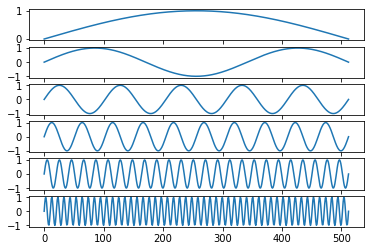
\includegraphics[width=\linewidth]{output_7_0.png}
  \end{center}
\end{frame}
\begin{frame}{Analysis of Jacobi}
  Now let's run 100 Jacobi iterations on each of the initial conditions,
  tracking the error at each iteration.
  \begin{center}
    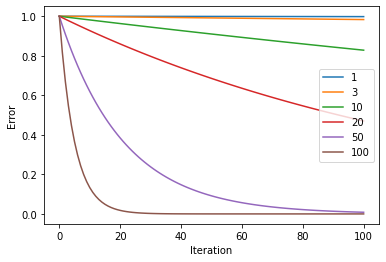
\includegraphics[width=\linewidth]{output_12_0.png}
  \end{center}

\end{frame}
\begin{frame}{Analysis of Jacobi}
  We can also look at our iterates:
  \begin{center}
    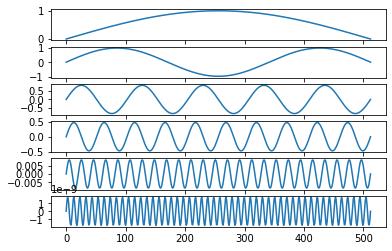
\includegraphics[width=\linewidth]{output_14_0.png}
  \end{center}
\end{frame}
\begin{frame}{Why Multigrid Works}
  Here we see the key to understanding the effectiveness of multigrid:

  Jacobi iteration is much better at eliminating high frequency error than low frequency error.
\end{frame}
\begin{frame}{How Do We Use This?}
  Notice what happens if we start with a low frequency wave and approximate it
  with half as many points:
  \begin{center}
    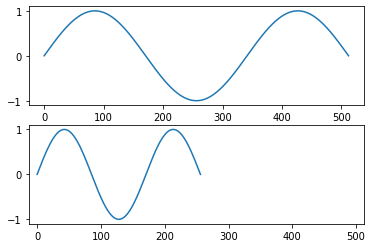
\includegraphics[width=\linewidth]{output_18_0.png}
  \end{center}
\end{frame}
\begin{frame}{How Do We Use This?}
  \begin{itemize}
  \item The same number of waves now fit into half the length
  \item Jacobi iteration is not aware of the physical structure of the
    problem
  \item For Jacobi, the shorter vector has higher frequency error than the
    longer vector
  \item Jacobi iteration could be more effective on this new shorter vector
  \end{itemize}
\end{frame}
\begin{frame}{Multigrid}
  As the name suggests, the multigrid method is about leveraging grids of
  different resolutions to take better advantage of Jacobi's convergence
  properties and computational effort.
\end{frame}
\begin{frame}{Notation}
  \begin{itemize}
  \item The $\Omega^h$ be the grid on which we wish to have a final approximation.
  \item Superscripts with interval length will be used to denote the grid a
    quantity is defined on
  \item For example $A^h$, $e^h$, $b^{h}$, $r^h$ are all used for the finest grid
  \item $A^{2h}$, $e^{2h}$, $b^{2h}$, $r^{2h}$ are all used for quantities on a grid
    with half the number of subintervals (thereby making their length $2h$)
  \end{itemize}
\end{frame}
\begin{frame}{Basic Multigrid Idea}
  \begin{itemize}
  \item Start with $k_1$ Jacobi iterations ($k_1$ small)
  \item We don't expect this iteration $x^h$ to be the exact solution
  \item Write exact solution with the form $x^* = x^{h} + e^{h}$
  \item Re-write the matrix system
    \begin{align*}
      A^h(x^h + e^h) &= b^h \\
      b^h - A^hx^h &= A^he^h = r^h
    \end{align*}
  \item On a coarser grid to solve $A^{2h}e^{2h} = r^{2h}$ and use that solution
    to estimate $e^h$
  \item Update $x^{h}$ as $x^h \leftarrow x^h + e^h$
  \item Run another $k_2$ iterations of Jacobi to smooth the error
  \end{itemize}
\end{frame}
\begin{frame}{Finding $e^h$}
  \begin{itemize}
  \item Want to solve $A^{2h}e^{2h} = r^{2h}$
  \item $A^{2h}, e^{2h}, r^{2h}$ are ``coarse grid versions'' of $A^h, e^h, r^h$.
  \item Smaller matrix $\Rightarrow$ less computation
  \item Low frequency error in $e^h$ $\Rightarrow$ higher frequency error in $e^{2h}$
  \item Then ``interpolate'' $e^{2h}$ back up to the finer grid
  \end{itemize}
\end{frame}
\begin{frame}{Moving Between Grids}
  \begin{itemize}
  \item In previous slides, I mentioned using the ``coarse grid versions'' of our
    quantities.
  \item We need to discuss how these quantities are obtained
  \item Assume coarse grid spacing which is twice as large as finer grid
  \item Almost universal practice - not evidence that any other ratio is more effective
  \end{itemize}
\end{frame}
\begin{frame}{Restriction Operator}
  \begin{itemize}
  \item For transforming fine grid vectors into coarse grid vectors 
  \item Denoted as $I_h^{2h}$
  \item Multiple Options
    \begin{itemize}
    \item Could simply remove every other entry
    \item More common - \textbf{full weighting}:\\
      Produce coarse grid vectors according to the rule \(I_{h}^{2h} x^{h} =
      x^{2h}\) where
      \begin{align*}
        x_{j}^{2h} &= \frac{1}{4} \left( x_{2j-1}^{h} + 2x_{2j} + x_{j+1}^{h} \right)
      \end{align*}
    \end{itemize}
  \end{itemize}
\end{frame}
\begin{frame}{Full Weighting}
  For example, if we have 7 interior nodes in the fine grid, and 3 interior nodes in
  the coarse grid, then we have the following: \[
    I_{h}^{2h} x^{h} = \frac{1}{4} 
    \begin{bmatrix}
      1 & 2 & 1 &   &   &   & \\
      &   & 1 & 2 & 1 &   & \\
      &   &   &   & 1 & 2 & 1 \\
    \end{bmatrix}
    \begin{bmatrix}
      x_1 \\ x_2 \\ x_3 \\ x_4 \\ x_5 \\ x_6 \\ x_7
    \end{bmatrix}_{h}
    = \begin{bmatrix}
      x_1 \\ x_2 \\ x_3
    \end{bmatrix}_{2h} = x^{2h}
  \]
  This opreator also has another advantage that we'll mention later.
\end{frame}
\begin{frame}{Full Weighting}
  \begin{center}
    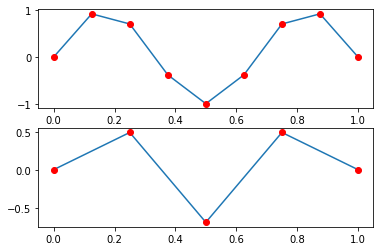
\includegraphics[width=\linewidth]{output_21_1.png}
  \end{center}
\end{frame}
\begin{frame}{Interpolation Operator}
  \begin{itemize}
  \item Also called the \textbf{Prolongation} operator
  \item Transforms coarse grid vectors into finer grid vectors
  \item Denoted as \(I_{2h}^h\)  
  \item Rule:\begin{align*}
               x_{2j}^h &= x_j^{2h} \\
               x_{2j+1}^h &= \frac{1}{2} \left( x_j^{2h} + x_{j+1}^{2h} \right)
             \end{align*}
  \item For shared grid points, let values coinside
  \item Generate additional fine grid points as average of
    surrounding coarse grid points
  \end{itemize}

\end{frame}
\begin{frame}{Prolongation Operator}
  \[
    I_{2h}^h x^{2h} = \frac{1}{2} 
    \begin{bmatrix}
      1 & & \\
      2 & & \\
      1 & 1 & \\
      & 2 & \\
      & 1 & 1 \\
      & & 2 \\
      & & 1
    \end{bmatrix}
    \begin{bmatrix}
      x_1 \\ x_2 \\ x_3 \\
    \end{bmatrix}_{2h}
    = \begin{bmatrix}
      x_1 \\ x_2 \\ x_3 \\ x_4 \\ x_5 \\ x_6 \\ x_7
    \end{bmatrix}_h = x^h
  \]
  \begin{itemize}
  \item Another advantage: \(I_{2h}^h = c(I_h^{2h})^T\)
  \item Important property for theory of multigrid
  \end{itemize}
\end{frame}
\begin{frame}{Prolongation Operator}
  \begin{center}
    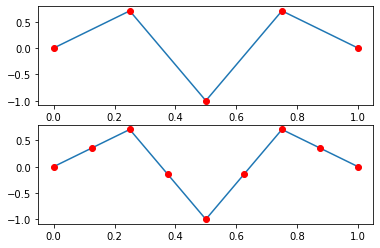
\includegraphics[width=\linewidth]{output_24_1.png}
  \end{center}
\end{frame}
\begin{frame}{Coarse Grid $A$}
  \begin{itemize}
  \item Two main methods:
    \begin{itemize}
    \item Generate discretization of the coarse grid problem
    \item \textbf{Galerkin Projection: }\[
        A^{2h} = I_h^{2h} A^h I_{2h}^h
      \]
    \end{itemize}
  \item With full weighting on 1D, both options are the same
  \end{itemize}
\end{frame}
\begin{frame}{Galerkin Projection}
  First, let \(e_j^{2h}\) denote the vector on the coarse grid with a 1 in
  the \(j\)th entry, and zeros elsewhere. Then \(A^{2h}e_j^{2h} = I_h^{2h}A^{h}I^h_{2h}e_j^{2h}\) will be
  the \(j\)th column of \(A^{2h}\). We will calculate this column in
  steps: \[
    I_{2h}^{h}e_j^{2h} =
    \frac{1}{2}
    \begin{bmatrix}
      1 &   &   & \\
      2 &   &   & \\
      1 & 1 &   & \\
      & 2 &   & \\
      & 1 & 1 & \\
      &   & 2 & \\
      &   & 1 & \ddots \\
      &   &   & \ddots \\
      &   &   & \ddots
    \end{bmatrix}
    \begin{bmatrix}
      0 \\ \vdots \\ 0 \\ 1 \\ 0 \\ \vdots \\ 0
    \end{bmatrix}
    =
    \begin{bmatrix}
      0 \\ \vdots \\ 0 \\ \frac{1}{2} \\ 1 \\ \frac{1}{2} \\ 0 \\ \vdots \\ 0
    \end{bmatrix}
  \]
\end{frame}
\begin{frame}{Galerkin Projection}
  Notice, this vector now lies in the fine grid so we can now apply the
  fine grid operator \(A^h\) to this vector:
  \begin{equation*}
    A^h I_{2h}^h e_j^{2h} =
    \frac{1}{h^2}
    \begin{bmatrix}
      2 & -1  &    &    & \\
      -1 & 2  & -1 &    & \\
      & -1 & 2  & -1 &  \\
      &    & \ddots & \ddots & \ddots
    \end{bmatrix}
    \begin{bmatrix}
      0 \\ \vdots \\ 0 \\ \frac{1}{2} \\ 1 \\ \frac{1}{2} \\ 0 \\ \vdots \\ 0
    \end{bmatrix} 
    = \begin{bmatrix}
      0 \\ \vdots \\ 0 \\ \frac{-1}{2h^2} \\ 0 \\ \frac{1}{h^2} \\ 0 \\ \frac{-1}{2h^2} \\ 0 \\ \vdots \\ 0
    \end{bmatrix}
  \end{equation*}
\end{frame}
\begin{frame}{Galerkin Projection}
  Finally, we apply the restriction operator to this vector to obtain a vector in the course grid space: \[
    I_{h}^{2h} A^{h} I_{2h}^h e_j^{2h} = \frac{1}{4}
    \begin{bmatrix}
      1 & 2 & 1 & & & & & & \\
      & & 1 & 2 & 1 & & & &  \\
      & & & & 1 & 2 & 1 & &  \\
      & & & &             &             & \ddots          & \ddots & \ddots \\
    \end{bmatrix}
    \begin{bmatrix}
      0 \\ \vdots \\ 0 \\ \frac{-1}{2h^2} \\ 0 \\ \frac{1}{h^2} \\ 0 \\ \frac{-1}{2h^2} \\ 0 \\ \vdots \\ 0
    \end{bmatrix}
    =
    \begin{bmatrix}
      0 \\ \vdots \\ 0 \\ \frac{-1}{4h^2} \\ \frac{1}{2h^2} \\ \frac{-1}{4h^2} \\ 0 \\ \vdots \\ 0
    \end{bmatrix}
  \] Notice that this is exactly the same column we obtain from creating discretization on the coarse grid.
\end{frame}
\begin{frame}{Galerkin Projection}
  This projection will not be the same
  as the coarse grid discretization in a 2D problem or if full weighting
  is not used. Nevertheless, it is a common practice and has been shown to
  produce good results. It also has the advantage that it requires no
  extra effort on the part of the user, it can simply be another step in
  the algorithm.
\end{frame}
\begin{frame}{Formal Two-Grid Cycle}
  (in Briggs, this is called a Coarse Grid Correction Scheme)
  \begin{enumerate}
  \item Relax \(\nu_1\) times on \(A^h x^h = b^h\) on \(\Omega^h\) with initial guess
    \(x^h\)
  \item Compute \(r^{2h} = I_h^{2h}(b^h - A^h x^h)\)
  \item Solve \(A^{2h} e^{2h} = r^{2h}\) on \(\Omega^{2h}\)
  \item Correct fine grid approximation: \(x^h \leftarrow x^h + I_{2h}^h e^{2h}\)
  \item Relax \(\nu_2\) times on \(A^h x^h = b^h\) on \(\Omega^h\) with initial guess
    \(x^h\)
  \end{enumerate}
\end{frame}
\begin{frame}[fragile]{Two-Grid Cycle}
\begin{lstlisting}[language=Python]
def TwoGridScheme(A_fine, b, numPreRelax, numPostRelax, numiters=1):
    I_Restrict = BuildFullWeighting(A_fine.shape[0])
    I_Prolong = 2*I_Restrict.T
    
    x = np.zeros_like(b)
    
    A_coarse = I_Restrict.dot(A_fine.dot(I_Prolong))
    
    for i in range(numiters):
        # First we relax on the fine grid:
        x = Jacobi(x, A_fine, b, numiters=numPreRelax) 
        
        # Now compute the restricted residual
        r_coarse = mvmult(I_Restrict, b - mvmult(A_fine, x)) 
    
        # Now we solve the coarse problem Ae = r using CG
        e_coarse = PCG(A_coarse, r_coarse, maxiter=100000)

        # Correct the fine-grid x with the prolongated residual
        x += mvmult(I_Prolong, e_coarse) 
    
        # Relax again
        x = Jacobi(x, A_fine, b, numiters=numPostRelax) 
    return x
\end{lstlisting}
\end{frame}
\begin{frame}{Testing Two-Grid Cycle}
  \begin{itemize}
  \item $N = 2^{16}$
  \item Generate random $x^*$ to manufacture $b$
  \item Start with initial $x_0 = 0$
  \end{itemize}
\end{frame}
\begin{frame}{Two Grid Results}
  \begin{tabular}{lcrr}
    Algorithm & Iter & Rel Error & Time (sec) \\
    \hline
    Jacobi                   & 100 &  0.87381  & 37.455 \\
    Two Grid (1 pre, 1 post) & 1	 &  0.29484  &  8.900 \\
    Two Grid (1 pre, 1 post) & 3	 &  0.23544  & 32.962 \\
    Two Grid (3 pre, 3 post) & 1	 &  0.23544  & 11.599
  \end{tabular}
  \begin{itemize}
  \item Can't read too much into the results yet
  \item Using CG for coarse level - maybe that's the speedup
  \item Last two lines give some hope though
  \end{itemize}

  Let's try:
  \begin{itemize}
  \item More relaxations pre and post
  \item CG for the fine grid problem
  \end{itemize}
\end{frame}
\begin{frame}{More Results}
  \begin{tabular}{lcrr}
    Algorithm & Iter & Rel Error & Time (sec) \\
    \hline
    Jacobi                   & 100   &  0.87381  & 37.455 \\
    Two Grid (1 pre, 1 post) & 1	   &  0.29484  &  8.900 \\
    Two Grid (1 pre, 1 post) & 3	   &  0.23544  & 32.962 \\
    Two Grid (3 pre, 3 post) & 1	   &  0.23544  & 11.599 \\
    Two Grid (5 pre, 5 post) & 1     &  0.20961  & 14.517 \\
    CG                       & 46078 &  0.21183  & 28.235
  \end{tabular}
  \begin{itemize}
  \item 2x speed-up to use Two Grid over straight CG
  \item More we can do to improve this
  \end{itemize}
\end{frame}
\begin{frame}{Recursion}
  Look at the Two-Grid Algorithm again:
  \begin{enumerate}
  \item Relax \(\nu_1\) times on \(A^h x^h = b^h\) on \(\Omega^h\) with initial guess
    \(x^h\)
  \item Compute \(r^{2h} = I_h^{2h}(b^h - A^h x^h)\)
  \item Solve \(A^{2h} e^{2h} = r^{2h}\) on \(\Omega^{2h}\)
  \item Correct fine grid approximation: \(x^h \leftarrow x^h + I_{2h}^h e^{2h}\)
  \item Relax \(\nu_2\) times on \(A^h x^h = b^h\) on \(\Omega^h\) with initial guess
    \(x^h\)
  \end{enumerate}
  Notice in step 3, we are just solving a smaller linear system.
  We can replace this solve with another course-grid correction, applying the
  same process to solve on that grid.

  Applying this idea \textbf{recursively} is a major concept behind the Multigrid
  method.  At each grid level, our matrix system gets exponentially smaller,
  allowing faster computation of the coarser levels.
\end{frame}
\begin{frame}{V-Cycle}
  There are several ways to construct a recursive multigrid pattern.

  The most common is the \textbf{V-Cycle}:
  \begin{center}
    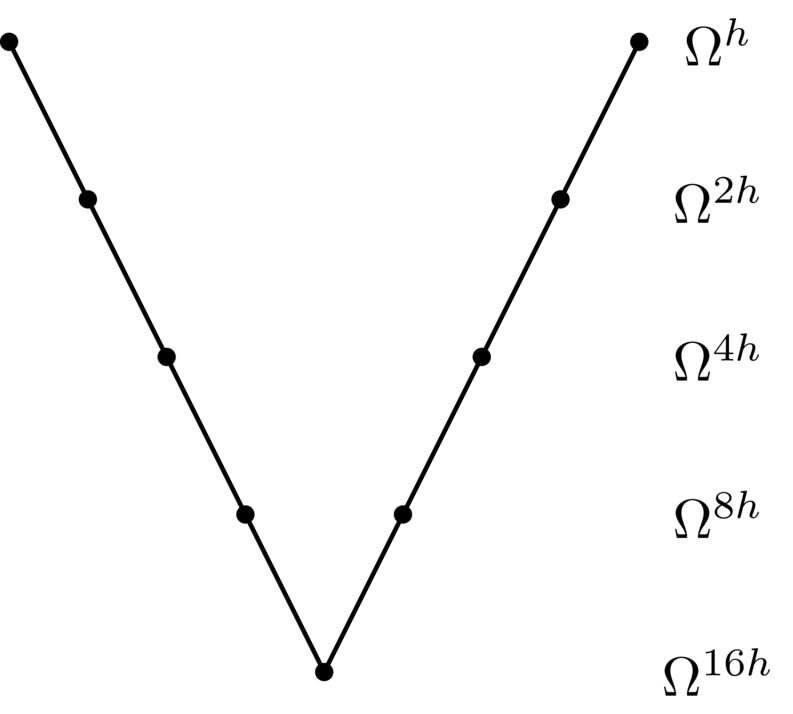
\includegraphics[height=2in]{../Graphics/V-Cycle-Graphic.png}
  \end{center}
\end{frame}
\begin{frame}[fragile]{V-Cycle}
  Here is the code - it's an adapted version of the Two-Grid above
\begin{lstlisting}[language=Python]
def VCycle(A_fine, b, numPreRelax, numPostRelax, coarsest_N, numiters=1):
    N = A_fine.shape[0]
    I_Restrict = BuildFullWeighting(N)
    I_Prolong = 2*I_Restrict.T
    
    A_coarse = I_Restrict.dot(A_fine.dot(I_Prolong))
    N_coarse = A_coarse.shape[0]
    
    for i in range(numiters):
        # First we relax on the fine grid:
        x = Jacobi(x, A_fine, b, numiters=numPreRelax)
    
        # Now compute the restricted residual
        r_coarse = mvmult(I_Restrict, b - mvmult(A_fine, x))
    
        # If not on the "bottom of the V", we call recursively
        if N_coarse > coarsest_N:
            # only 1 iteration to get the V-Cycle
            e_coarse = VCycle(A_coarse, r_coarse, numPreRelax, numPostRelax, coarsest_N, 1)
        else: # If on the bottom of the V, we solve the coarsest matrix exactly
            e_coarse = PCG(A_coarse, r_coarse, maxiter=100000)
    
        # Correct the fine-grid x with the prolongated residual
        x += mvmult(I_Prolong, e_coarse)
    
        # Relax Again
        x = Jacobi(x, A_fine, b, numiters=numPostRelax)
    
        return x
\end{lstlisting}
  \end{frame}
  \begin{frame}{V-Cycle Results}
    \begin{table}
      \scriptsize
      \begin{tabular}{lcrr}
        Algorithm & Iter & Rel Error & Time (sec) \\
        \hline
        Jacobi                                  & 100   &  0.87381  & 37.455 \\
        Two Grid (1 pre, 1 post)                & 1	    &  0.29484  &  8.900 \\
        Two Grid (1 pre, 1 post)                & 3	    &  0.23544  & 32.962 \\
        Two Grid (3 pre, 3 post)                & 1	    &  0.23544  & 11.599 \\
        Two Grid (5 pre, 5 post)                & 1     &  0.20961  & 14.517 \\
        CG                                      & 46078 &  0.21183  & 28.235 \\
        V-Cycle (3 pre, 3 post, 127x127 coarse) & 1     &  0.23201  & 4.7490 \\
        V-Cycle (3 pre, 3 post, 127x127 coarse) & 3     &  0.18222  & 13.906 \\
        V-Cycle (5 pre, 5 post, 127x127 coarse) & 1     &  0.20767  & 7.6766
      \end{tabular}
    \end{table}
    These are looking pretty good, but the coarse grid size above was chosen
    arbitrarily.  Let's test and see if we can find an optimal coarse grid size
  \end{frame}
  \begin{frame}{Stopping Analysis}
    All trials are single V-Cycle run with 5 pre and 5 post relaxations
    \begin{table}
      \begin{tabular}{crr}
        Coarse Matrix Size & Rel Error & Time (sec) \\
        \hline
        3x3         & 0.20863 & 7.64522 \\
        7x7         & 0.20801 & 7.70789 \\
        15x15       & 0.20784 & 7.62153 \\
        31x31       & 0.20774 & 7.64096 \\
        63x63       & 0.20768 & 7.68061 \\
        127x127     & 0.20767 & 7.65519 \\
        255x255     & 0.20766 & 7.82747 \\
        511x511     & 0.20767 & 7.94081 \\
        1023x1023   & 0.20770 & 8.07504 \\
        2047x2047   & 0.20777 & 7.64995 \\
        4095x4095   & 0.20790 & 7.38173 \\
        8191x8191   & 0.20816 & 7.14767 \\
        16383x16383 & 0.20868 & 8.89681 \\
        32767x32767 & 0.20961 & 14.0686
      \end{tabular}
    \end{table}
  \end{frame}
  \begin{frame}{Overall Results}
    \begin{table}
      \scriptsize
      \begin{tabular}{lcrr}
        Algorithm & Iter & Rel Error & Time (sec) \\
        \hline
        Jacobi                                    & 100   &  0.87381  & 37.455 \\
        Two Grid (1 pre, 1 post)                  & 1	    &  0.29484  &  8.900 \\
        Two Grid (1 pre, 1 post)                  & 3	    &  0.23544  & 32.962 \\
        Two Grid (3 pre, 3 post)                  & 1	    &  0.23544  & 11.599 \\
        Two Grid (5 pre, 5 post)                  & 1     &  0.20961  & 14.517 \\
        CG                                        & 46078 &  0.21183  & 28.235 \\
        V-Cycle (3 pre, 3 post, 127x127 coarse)   & 1     &  0.23201  & 4.7490 \\
        V-Cycle (3 pre, 3 post, 127x127 coarse)   & 3     &  0.18222  & 13.906 \\
        V-Cycle (5 pre, 5 post, 127x127 coarse)   & 1     &  0.20767  & 7.6766 \\
        V-Cycle (5 pre, 5 post, 8191x8191 coarse) & 1     &  0.20816  & 7.1476
      \end{tabular}
    \end{table}
  \end{frame}
  \begin{frame}{More Iterations}
    Run 5 pre, 5 post 8191x8191 coarse grid V-Cycle for 30 iterations, tracking
    error:
    \begin{center}
      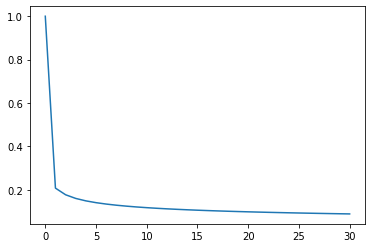
\includegraphics[height=1.5in]{output_41_1.png}
    \end{center}
    Notice the large decrease in error (80\% reduction) after the first iteration.
    This is one of the primary reasons why multigrid tends to make a good preconditioner.

  \end{frame}
  \begin{frame}{W-Cycle}
    Complete two V-Cycles on every recursive call:
    \begin{center}
      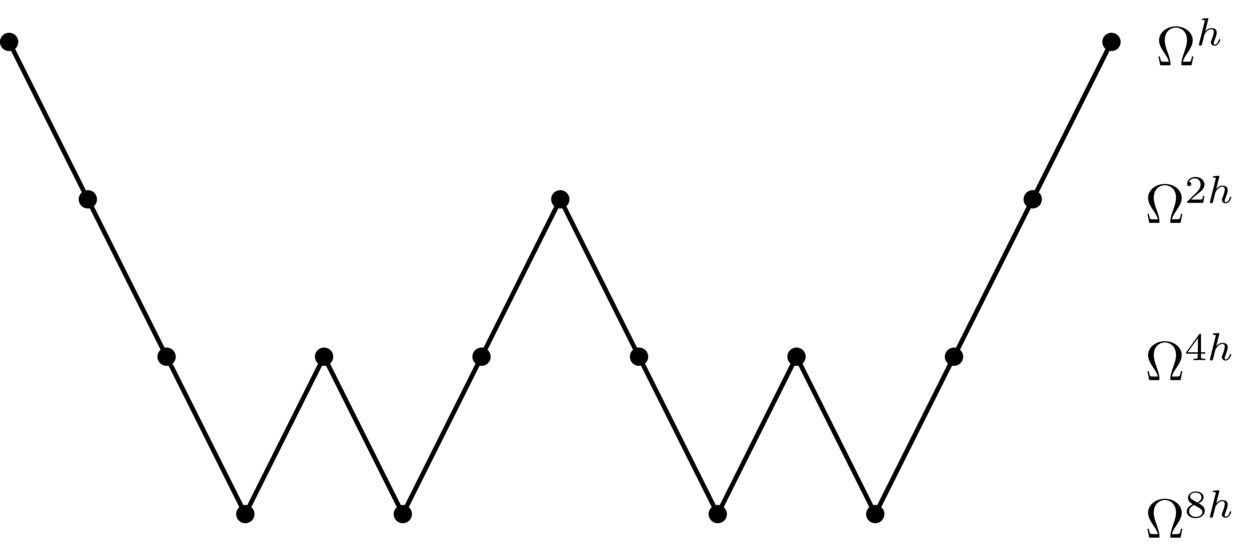
\includegraphics[height=1.8in]{../Graphics/W-Cycle-Graphic.png}
    \end{center}
    Generalizes to what Briggs calls $\mu$-Cycles, where you complete $\mu$ V-Cycles
    on every recursive call. Values of $\mu \geq 3$ are not common.
  \end{frame}
  \begin{frame}{Full Multigrid Cycle}
    \begin{center}
      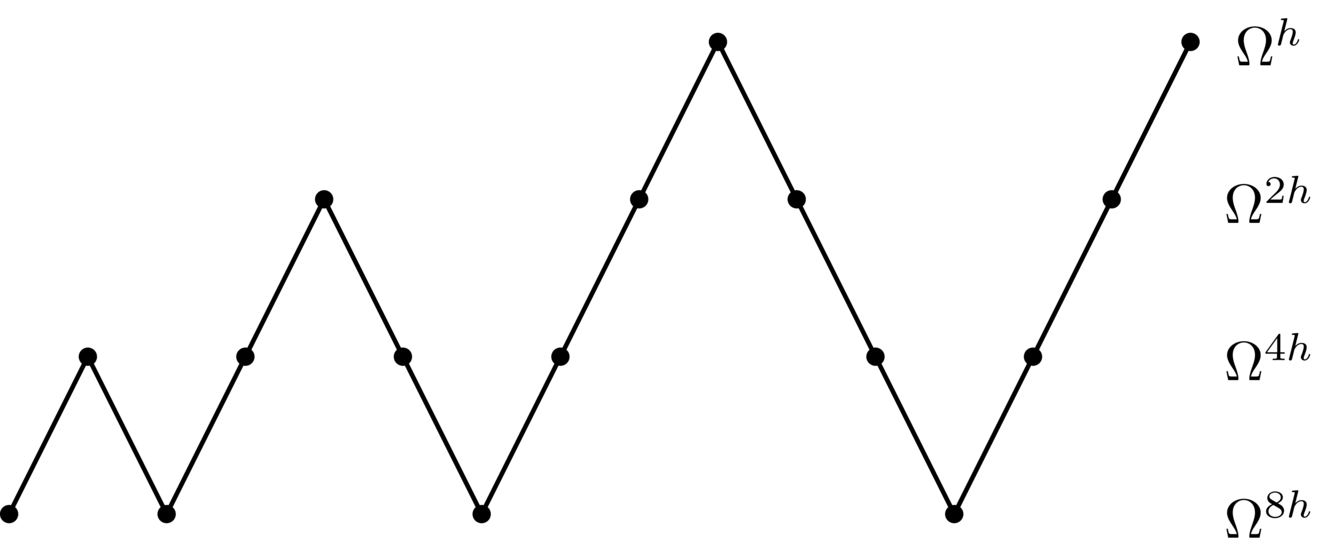
\includegraphics[height=1.8in]{../Graphics/FMV-Cycle-Graphic.png}
    \end{center}
    \begin{enumerate}
    \item Get good initial guess on coarsest grid, correct next finer grid
    \item Run a V-Cycle to get a better initial guess for next level up
    \item Keep doing V-Cycles until the finest grid is solved
    \end{enumerate}
  \end{frame}
  \begin{frame}{Choices to Make}
    \begin{itemize}
    \item Relaxation method
      \begin{itemize}
      \item Weighted Jacobi (or other variations of Jacobi)
      \item Gauss-Seidel (or variations of it)
      \item Red-Black versions of Jacobi and GS have been studied
      \item Block Jacobi and GS are options as well
      \end{itemize}
    \item Coarse grid solver
    \item Number of relaxations (typically 3-5 pre and post)
    \item Cycle to use (V-Cycle is most common)
    \end{itemize}
  \end{frame}
  \begin{frame}{Algebraic Multigrid}
    \begin{itemize}
    \item Geometric multigrid is useful for gaining intuition into multigrid
      methods, but not often used in practice
    \item For general meshes, much tougher to create the restriction and
      prolongation operators
    \item Only the physical dimensions are reduced on coarser grid
    \end{itemize}
    \vspace{.2in}
    Algebraic multigrid is a similar method that depends on the coefficient
    matrix, not the underlying geometric structure.
  \end{frame}
  \begin{frame}{Algebraic Multigrid}
    \begin{equation*}
      A = \frac{1}{h^2}
      \begin{bmatrix}
        2  & -1 &        &        &        &   \\
        -1 &  2 & -1     &        &        &   \\
        & -1 &  2     &     -1 &        &   \\
        &    & \ddots & \ddots & \ddots &   \\
        &    &        &     -1 &      2 & -1 \\
        &    &        &        &     -1 &  2
      \end{bmatrix}
    \end{equation*}
    \begin{itemize}
    \item Interpret the magnitudes of the values in the matrix as their ``contribution''
      in calculating the element on the diagonal.
    \item Use this idea of ``significance'' to determine which unknowns in the
      matrix can be ``merged'' to obtain a ``coarser'' matrix problem
    \item This process creates prolongation and restriction operators that only
      depend on the matrix, not the geometric structure
    \end{itemize}

  \end{frame}
  \begin{frame}{Algebraic Multigrid}
    Algebraic multigrid can be programmed in a much more general way and
    can be more easily extended to other problems.  This also makes it more useful
    as a preconditioner.
  \end{frame}
  \begin{frame}{Questions?}
  \end{frame}
\end{document}
